\chapter{Terminology and Preliminaries}\label{ch:prelim}

\vspace*{-50pt}

\begin{figure}[ht]
        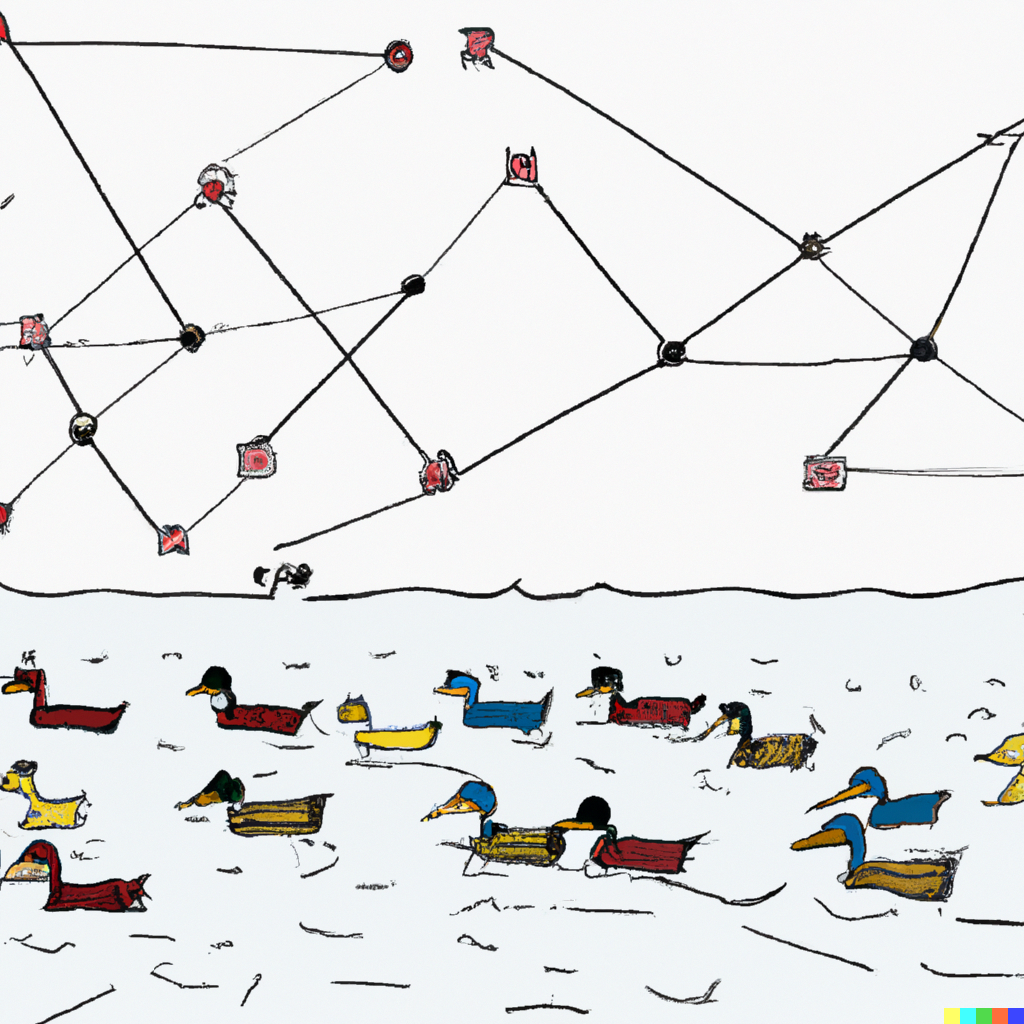
\includegraphics[width=0.35\textwidth, right]{img/gt-ducks.png}
        \captionsetup{textformat=empty,labelformat=blank}
        \caption{Generated with Dall-E. \url{https://labs.openai.com/}. ``Ducks learning graph theory while swimming on a sea sketched in color complex''}
\end{figure}

\epigraph{\itshape ``All we have to decide is what to do with the time that is given to us.''}{J. R. R. Tolkien, \textit{Gandalf} in \textit{Lord of the Rings}}


In this chapter, we will introduce the core definitions used throughout this thesis. 
Most of the definitions of graph theory are taken from Diestel \cite{Diekert2005}. 
For definitions in the area of \textit{parameterized complexity}, the book by Cygan et al.\cite{Cygan2015} gives a very good introduction.
For standard mathematical notation, the reader is referred to any introductory textbook into discrete maths (e.g. \cite{Rosen2012}).

\section{Graph Theory}

If not explicitly stated otherwise, the following definitions are taken from the book \textit{Graph Theory} written by Reinhard Diestel \cite{diestel10}.

\subsection{Basic Terminology}

\begin{definition}[Graph]
    A simple graph is a pair $G = (V, E)$ of two sets where $V$ denotes the vertices and $E \subseteq V \times V$ the edges of the graph.  A vertex $v \in V$ is incident with an edge $e \in E$ if $v \in e$. Two vertices $x, y$ are adjacent, or neighbours, if $\{x,y \} \in E$. By this definition, graph loops and multiple edges are excluded.
    
    A multigraph is a pair $(V, E)$ of disjoint sets together with a map $E \rightarrow V \cup [V]^2$ assigning to every edge either one or two vertices, its ends. Multigraphs can have loops and multiple edges.
    
    We usually denote the vertex set by $V(G)$ and its edge set by $E(G)$.


    % TODO connected 

\end{definition}

Unless stated otherwise, we usually consider only \textit{simple graphs}, but the notion of \textit{multigraphs} gets important when we later talk about the \textit{underlying multigraph} of a \dreg. 

\begin{definition}[Subgraph and Induced Subgraph]
    Let \G and $G' = (V', E')$ be two graphs. If $V' \subseteq V$ and $E' \subseteq E$ then $G'$ is a \underline{subgraph} of $G$. 
    If $G$ is a subgraph of $G'$ and $G'$ contains all the edges to $G$ with both endpoints in $V(G')$, then $G'$ is an \underline{induced subgraph} of $G$ and we write $G' = G[V(G')]$.
\end{definition}


%TODO Quote
\begin{definition}[Degrees]
    Let \G be a graph. The \textit{degree} $d_G(v)$ (shortly $d(v)$ if $G$ is clear from the context) of a vertex $v \in V$ is the number of neighbors of v. We call a vertex of degree $0$ as \underline{isolated} and one of degree $1$ as a \underline{pendant}. If all the vertices of $G$ have the same degree $k$, then $g$ is $k$-regular.
\end{definition}

% TODO Quote e.g. The open neighborhood number of a graph
\begin{definition}[Closed and Open Neighborhoods {\cite{Balakrishnan2012}}]
    Let \G be a (non-empty) graph. 
    The set of all neighbors of $v$ is the \underline{open neighborhood} of $v$ and denoted by $N(v)$; the set $N[v] = N(v) \cup \{v\}$ is the \underline{closed neighborhood} f $v$ in $G$. When G needs to be made explicit, those open and closed neighborhoods are denoted by $N_G(v)$ and $N_G[v]$. 
\end{definition}

\begin{definition}[isomorphic Graphs]
Let \G and $G' = (V', E')$ be two graphs. We call $G$ and $G'$ \underline{isomorphic}, if there exists a bijection $\phi: V \rightarrow V'$ with $\{x, y\} \in E \Leftrightarrow \phi(x)\phi(y) \in E'$ for all  $x,y \in V$. Such a map $\phi$ is called \underline{isomorphism}.

If a graph $G$ is isomorphic to another graph $h$, we denote $G \simeq H$. 
\end{definition}

\begin{definition}[Paths and Cycles]
    A path is a non-empty graph $P = (V,E)$ of the form $V = \bigcup_{i  \in [k]} \{x_i\}$ and $E = \bigcup_{i \in  [k-1]} \{x_ix_{i+1}\}$ where the $x_i$ are distinct. The vertices $x_0$ and $x_k$ are \underline{linked} by $P$ and are called the \textit{ends} of $P$. The \underline{length} of a path is its number of edges and the path on $n$ vertices is denoted by  $P_n$. We refer to a path $P$ by a natural sequence of its vertices: $P = x_0x_1...x_k$. Such a path $P$ is a path between $x_0$ and $x_k$, or a $x_0,x_k$-path.
    If $P = x_0...x_k$ is a path and $k \geq 2$, the graph with vertex set $V(P)$ and edge set $E(P) \cup \{x_kx_0\}$ is a \underline{cycle}. The cycle on $n$ vertices is denoted as $C_n$.
    The \underline{distance} $d_G(v,w)$ from a vertex $v$ to a vertex $w$ in a graph $g$ is the length of the shortest path between $v$ and $w$. If $v$ and $w$ are not linked by any path in $G$, we set $d_G(v,w) = \infty$. Again, if $G$ is clear from the context, we omit the subscripted $G$ and just write $d(v,w)$ instead.
\end{definition}

\subsection{Graph Classes}

A \textit{graph class} is a set of graphs $\mathfrak{G}$ that is closed under isomorphism that is if $G \in \mathfrak{G}$ and a $H \simeq G$ then $H \in \mathfrak{G}$ as well.

\begin{definition}[Graph Parameters]
Let \G be a graph.
An  \underline{independent set} of $G$ is a set of pairwise non-adjacent vertices. 
A \underline{clique} of $G$ is a set of pairwise adjacent vertices. 
A \underline{vertex cover} of $G$ is a subset of vertices containing at least one endpoint of every edge. 
A \underline{dominating set} is a subset $D$ of vertices such that all vertices not contained in are adjacent to some vertex in $D$.
\end{definition}

\begin{graphclass}[r-partite]
    Let $r \geq 2$ be an integer. A Graph $G = (V, E)$ is called \underline{r-partite} if $V$ admits a partition into $r$ classes such that every edge has its ends in different classes: Vertices in the same partition class must not be adjacent. 
    A \textit{$2$-partite} graph is called \underline{bipartite}. 
    
    An $r$-partite graph in which every two vertices from different partition classes are adjacent is called \underline{complete}. For the \underline{complete bipartite graph} on bipartitions $X \uplus Y$ of size $m$ and $n$, we shortly write $K_{m,n}$. 
\end{graphclass}

\begin{graphclass}[Complete]
If all vertices of a graph \G are pairwise adjacent, we say that $G$ is \underline{complete}. 
A complete graph on $n$ vertices is a $K_n$. A $K_3$ is called a \underline{triangle}.
\end{graphclass}


%\begin{definition}[{\cite[IV. Triangulated Graphs]{Berge1966}}]
%    A graph G is called \textit{chordal} (or in the older literature \textit{triangulated}) graphs if for every cycle $c = [p_1,...,p_n,p_1]$ of length $l > 3$ there is an edge of $G$ joining two non-consecutive vertices of c. Such vertices are called chords of the cycle   
%\end{definition}

\begin{graphclass}[Chordal]
For a graph \G, an edge that joins two vertices of a cycle, but is not itself an edge of the cycle is a \underline{chord} of that cycle.

Furthermore, we say $G$ is \underline{chordal} (or \textit{triangulated}) if each of its cycles of length at least four has a chord. In other words, it contains no induced cycle other than triangles.

\end{graphclass}

\begin{graphclass}[Split]
A \underline{split graph} is a graph \G whose vertices can be partitioned into a clique and an independent set.    
\end{graphclass}

%\begin{graphclass}[Bipartite {\cite[p.5]{Bondy2008}}]
%A \textit{\bg} is a Graph G whose vertex set can be partitioned into two subsets X and Y, so that each edge has one end in X and one end in Y. Such a partition (X,Y) is called a \textit{bipartition} of G.
%\end{graphclass}

%\begin{definition}[Perfect Graphs]
    
%\end{definition}

\begin{graphclass}[Planar]

A \textit{plane graph} is a pair $(V,E)$ of finite sets with the following properties:

\begin{itemize}
    \item $V \subseteq \mathbb{R}^2$ (Vertices).
    \vspace{-2mm}
    \item Every edge is an arc between two vertices, 
    \vspace{-2mm}
    \item different edges have different sets of endpoints, and
    \vspace{-2mm}
    \item The interior of an edge contains no vertex and no point of any other edge
\end{itemize}

An embedding in the plane, or \textit{planar embedding}, of an (abstract) graph $G$ is an isomorphism between $G$ and a plane graph $H$. A \textit{plane graph} can be seen as a concrete \textbf{embedding} of the planar graph into the ``plane'' $\mathbb{R}^2$.

\end{graphclass}

For an introduction into classical complexity theory. Refer to the standard textbooks aaran und cpo.
Rely an \cite[]{}
\section{Parametrized Complexity}

\paragraph{Ways to cope with NP-hard problem} Usually 

\begin{center}
    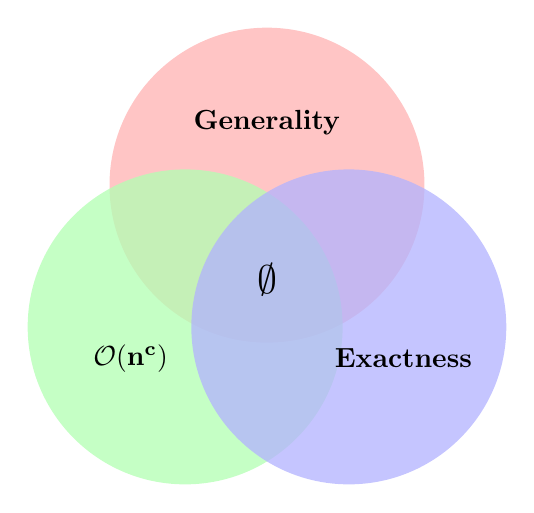
\begin{tikzpicture}
        \begin{scope}[blend mode = normal,opacity=0.75]
            \fill[red!30!white]   ( 90:1.2) circle (2);
            \fill[green!30!white] (210:1.2) circle (2);
            \fill[blue!30!white]  (330:1.2) circle (2);
        \end{scope}
        \node at ( 90:2)    {\textbf{Generality}};
        \node at ( 210:2)   {$\mathbf{\mathcal{O}(n^c)}$};
        \node at ( 330:2)   {\textbf{Exactness}};
        \node [font=\Large] {$\emptyset$};
    \end{tikzpicture}
\end{center}


\begin{definition}[Parametrized Problem{\cite[Def 1.1]{Cygan2015}}]
    A parametrized problem is a $L\subseteq\Sigma^*\times \mathbb{N}$ ($\Sigma$ finite fixed alphabet) for an instance $(x,k)\in \Sigma^*\times \mathbb{N}$, where k is called the \textit{parameter}.
\end{definition}

\begin{definition}[Instance Size]
    The \textbf{size of an instance} of an instance $(x,k)$ of a parametrized problem is $\abs{(x,k)} = \abs{x} + k$
\end{definition}
We will now clarify the basic terminology withing Parametrized Complexity. 
We are now giving a short introduction into the world of parametrized complexity. 
* General Introduction


\subsection{Fixed Parameter Tractability}

\begin{definition} [The Class FPT {\cite[Def 1.2]{Cygan2015}}]
    A parametrized problem $L\subseteq\Sigma^*\times\mathbb{N}$ is called \textit{fixed-parameter tractable} if there exists an algorithm A (called a \textit{fixed-parameter algorithm}), a computable function $f:\mathbb{N} \rightarrow \mathbb{N}$ and a constant c such that, given $(x,k) \in \Sigma^* \times \mathbb{N}$, the algorithm $\mathcal{A}$ correctly decides whether $(x,k) \in L$ in time bounded by $f(k) \cdot |(x,k)|^c$. The complexity class containing all fixed-parameter tractable problems is called \textit{FPT}
\end{definition}


\subsection{Kernelization}

\begin{definition}[kernelization Algoritm{\cite[Def 2.1]{Cygan2015}}]
A \textit{Kernelization Algorithm} or \textit{kernel} is an algorithm $\mathfrak{A}$ for a parametrized Problem Q, that given an instance $(I,k)$ of Q works in polynomial time and returns an equivalent instance $(I', k')$ of Q. Moreover, we require that $size_{\mathfrak{A}}(k) \leq g(k)$ for some computable function $g:\mathbb{N} \rightarrow \mathbb{N}$
\end{definition}

%TODO better
If we bound the size of the kernel by linear function $f(m) = \mathcal{O}(k)$, we say that the problem admits a \textbf{linear kernel}. 

%Examplary, if we reduce a graph for a graph problem in such a way that we can garuantee that our reduced graph only has a a few vertices \textbf{linear} in  $k$ left

The main idea, preprocessing algorithm, shrink size as much as possible, sound reduction rules,small output instance

\begin{definition}[Output size of a Preprocessing Procedure {\cite[p. 18]{Cygan2015}}] The output size of a preprocessing algorithms $\mathfrak{A}$ is defined as 

    \[\mathrm{size}_{\mathfrak{A}}(k) = \sup\{\abs{I'} + l': (I',k')= \mathfrak{A}(I,k), I \in \Sigma^* \} \]
\end{definition}

possibly infinite

Clearly, if there exists a kernelization algorithm for a problem $L$ and an algorithm $\mathfrak{A}$ with any runtime to decide $L$, the problem is in $FPT$ because after the kernelization pre-processing has been applied, the size of the reduced instance is a function merely in $k$ and independent of the input size $n$. In \cref{ch:linkern} we will explicitly construct a kernel for \psdom and hence showing it to be in \textit{FPT}. 

% Interstingly, als the converse?

\begin{definition}[Reduction Rules {\cite[p. 18]{Cygan2015}}]
A \textbf{reduction rule} is a function $\phi:\Sigma^* \times \mathbb{N} \rightarrow \Sigma^* \times \mathbb{N}$ that maps an instance $(x,k)$ to an equivalent instance $(x',k')$ such that $phi$ is computable in time polynomial in $\abs{x}$ and $k$
\end{definition}

\begin{definition}[Equivalent Instance {\cite[p. 18]{Cygan2015}}]
     This is a test
\end{definition}

\begin{definition}{Soundness of a rule}

\end{definition}

A \textbf{reduction rule} is a function $\Sigma* \times \mathbb{N}$ that maps an instance $(x,k)$ to an equivalent instance $(x',k')$ such that xx is computable in time polynomial in $\abs{x}$ and $k$

\subsection{Fixed Parameter Intractability: The w-Hierarchy}
\subsection{Compare to classical NP-Hardness theory}

\subsubsection{Parametrized Reductions}
\begin{definition}[Parametrized Reduction {\cite[Def 13.1]{Cygan2015}}] Let $A,B\subseteq \Sigma^*\times\mathbb{N}$ two parametrized problems. A \textit{Parametrized Reduction} from A to B is an algorithm that, given an instance $(x,k)$ of A, outputs an instance $(x', k')$ of B such that

    \begin{itemize}
        \item $(x,k)$ is a \textcolor{gray}{yes instance} of A \textbf{iff} $(x',k')$ is a \textcolor{gray}{yes instance} of B
        \item $k' \leq g(k)$ for some computable function $g$
        \item the running time is $f(k)\cdot |x|^{\mathcal{O}(1)}$ (FPT!)
    \end{itemize}
\end{definition}
    \subsubsection{The $w$-hierarchy}



\chapter{On parameterized Semitotal Domination}\label{ch:semitotal-domination}

\vspace*{-50pt}

\begin{figure}[ht]
        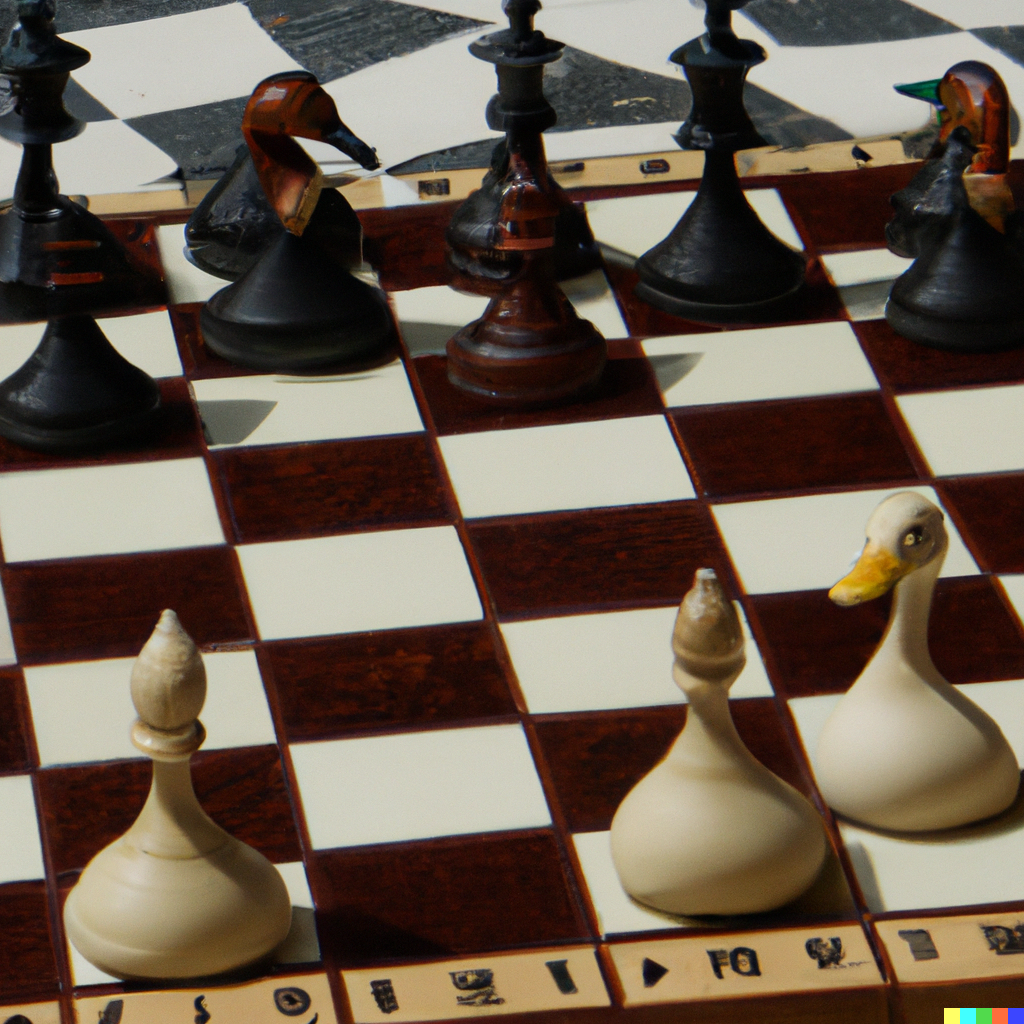
\includegraphics[width=0.35\textwidth, right]{img/chess.png}
        \captionsetup{textformat=empty,labelformat=blank}
        \caption{Generated with Dall-E. \url{https://labs.openai.com/}. ``Duck playing chess''}
\end{figure}

\epigraph{\itshape Todo select another quote}{Lewis Caroll, \textit{XXXX}}

In connection with various chessboard problems, the concept of domination can be traced back to the mid-1800s.
For example, de Jaenosch attempted in 1862 to solve the minimum number of queens required to fully cover an n x n-chessboard \cite{Jaenisch1862}. Because of the immense amount of publications related to domination, Haynes, Hedetniemi, and Slater started a comprehensive survey of the literature \cite{Haynes1998, Haynes1998b}. 
20 years later, by a series of three more books, Haynes, Henning and Hedetniemi updated the survey with the latest developments \cite{Haynes2020, Haynes2021, Haynes2022}.

After introducing the problem, we will dedicate the rest of this chapter to giving a current status about the complexity status of \dom, \sdom and \tdom on various graph classes. 
% Surprisingly, there are cases where the complexity of \dom and \tdom differes (e)
%If both \dom and \tdom are already hard for a class, we already have a strong assumption that this also holds for \sdom as well.


%Interestingly, most of them mimic each other for one specific class, but there are some exceptions, where this is not the case.

\section{The Domination Problem}

\textit{Semitotal domination} was introduced by Goddard, Henning and McPillan \cite{Goddard2014} as a relaxed form of \textit{total domination}. 

\begin{prb}[DOMINATING SET DECISION {\cite[p. 586]{Cygan2015}}]{prb:ds}
    \begin{tabularx}{0.9\textwidth}{>{\hsize=0.30\hsize}X>{\hsize=0.8\hsize}X}
        \textbf{Input:} & Graph \G and an integer $k$\\
        \textbf{Question:} & Is there a set $X \subseteq V$ of size at most $k$ such that $N[X] = V$? \\
    \end{tabularx}
\end{prb}


Goddard, Henning and McPiallan a

\begin{prb}[SEMITOTAL DOMINATING SET DECISION {\cite{Goddard2014}}]{prb:tds}
    
    \begin{tabularx}{0.8\textwidth}{>{\hsize=0.35\hsize}X>{\hsize=0.8\hsize}X}
        \textbf{Input:} & Graph \G and an integer $k$\\
        \textbf{Question:} & Is there a subset $X \subseteq V$ of size at most $k$ such that $N[X] = V$ and for all $d_1 \in X$ there exists another $d_2 \in X$ such that $d(d_1, d_2) \leq 2$?\\
    \end{tabularx}
        
\end{prb}

\begin{prb}[TOTAL DOMINATING SET DECISION {\cite[p. 596]{Cygan2015}}]{prb:sds}
    \begin{tabularx}{0.8\textwidth}{>{\hsize=0.35\hsize}X>{\hsize=0.8\hsize}X}
        \textbf{Input:} & Graph \G and an integer $k$\\
        \textbf{Question:} & Does there exists a set $X \subseteq V$ of at most $k$ vertices of G such that for every $u \in V(G)$ there exists $v \in X$ with $\{u,v\} \in E$ \\
    \end{tabularx}
        
\end{prb}

\begin{figure}
     \begin{equation*}
         \tikzfig{fig/tikz/ds-examples}
     \end{equation*}
    \caption[An example for various dominating sets]{\textit{An example for a dominating set, semitotal dominating set and a total dominating set, where $\gamma(G) < \gamma_{2t}(G) < \gamma_t(G)$ are strict. In the first case, only two vertices suffice to dominate all others. In the second one, we need a witness between $d_1$ and $d_2$ that is at most distance two. In the last case, $d_1$ and $d_2$ both need a neighbor in the total dominating set.}}
    \label{figd:dsexamples}
\end{figure}


\begin{definition}[Domination Parameters]
   The \underline{domination number} in a graph $G$ is the minimum cardinality of a dominating set of $G$, denoted as $\gamma(G)$. 
   The \underline{total domination number} is the minimum cardinality of a total dominating set (tds) of $G$, denoted by $\gamma_t(G)$.
   The \underline{semitotal domination number} is the minimum cardinality of a semitotal dominating set (sds) of $G$, denoted by $\gamma_t(G)$
\end{definition}

% Henning?


Since every total dominating set is also a semitotal dominating set and every semitotal dominating set is also a dominating set , we have the following fact first observed by Goddard and Henning \cite{Goddard2014}. 

\begin{fact}
For every graph $G$ with no isolated vertex, $\gamma(G) \leq \gamma_{t2}(G) \leq \gamma_t(G)$
\end{fact}

We can see that the semitotal domination number $\gamma_{t2}$ is squeezed between the \textit{domination} number and the \textit{total domination} number. It turns out that for some graphs, all of these inequalities can be strict. See \cref{figd:dsexamples} for an example, where $\gamma(G) < \gamma_{t2} < \gamma_t(G)$.

\subsection{Preliminaries}

* Witness
* u pendant ofrom a vertex c if $N(u) = \{w\}$
* domination 

Let $D$ be a dominating set of G and $w \in V(G) \setminus D$. For any neighbor $v \in D \cap N(w)$, we say that $d_1$ \textit{dominates} $w$ For two dominating vertices $d_1, d_2in D$. If 

Definition, dominating number

\section{Complexity Status of \sdom}\label{ch:complexity-status}

% Surprisingly, there are cases where the complexity of \dom and \tdom differes (e)
%If both \dom and \tdom are already hard for a class, we already have a strong assumption that this also holds for \sdom as well.

\section{\hmath $w[i]$-Intractibility}

Now some w[i] hard classes. 

\subsection{Warm-Up: \hmath $W[2]$-hard on General Graphs}

% TODO can we conclude anything for AT Free Graphs?
%% TODO Extend to r-partite

As any \bg with bipartition can be split further into \rpg this results also implies the \wone-hardness of \rpg

